% lec note: https://docs.google.com/document/d/1mhnFaNrPPQxUFme8OVD2Y1bqOOBA-wp7/edit

% lit table: https://docs.google.com/spreadsheets/d/18b49O5U6Iusc4eWiq-ptuGLScmuvRLM1R2cAtGL4iBk/edit#gid=0

% draft shown to Gugsi with comments: https://drive.google.com/file/d/1-VRO2d18OMNqKiyVQiU3uFEhnkt4wf_s/view
% ---------

\section{Chapter Overview}
% 1/4 pg
As mentioned in the introduction chapter, \gls{nft}s have been a very popular application of Blockchain in the recent months. In this chapter, the author critiques on related work with respect to the application of Recommendation Systems while further exploring what, why \& how \gls{nft}s have been making the headlines and pulling in investors from around the globe. Furthermore, the author has brought-forward possible improvements that may open up possibilities of providing expected recommendations in the \gls{nft}-space.

\section{Concept Map}
% 1/4 pg + Appendix
\nameref{appendix:A}

% \begin{figure}[h!]
% \centering
% 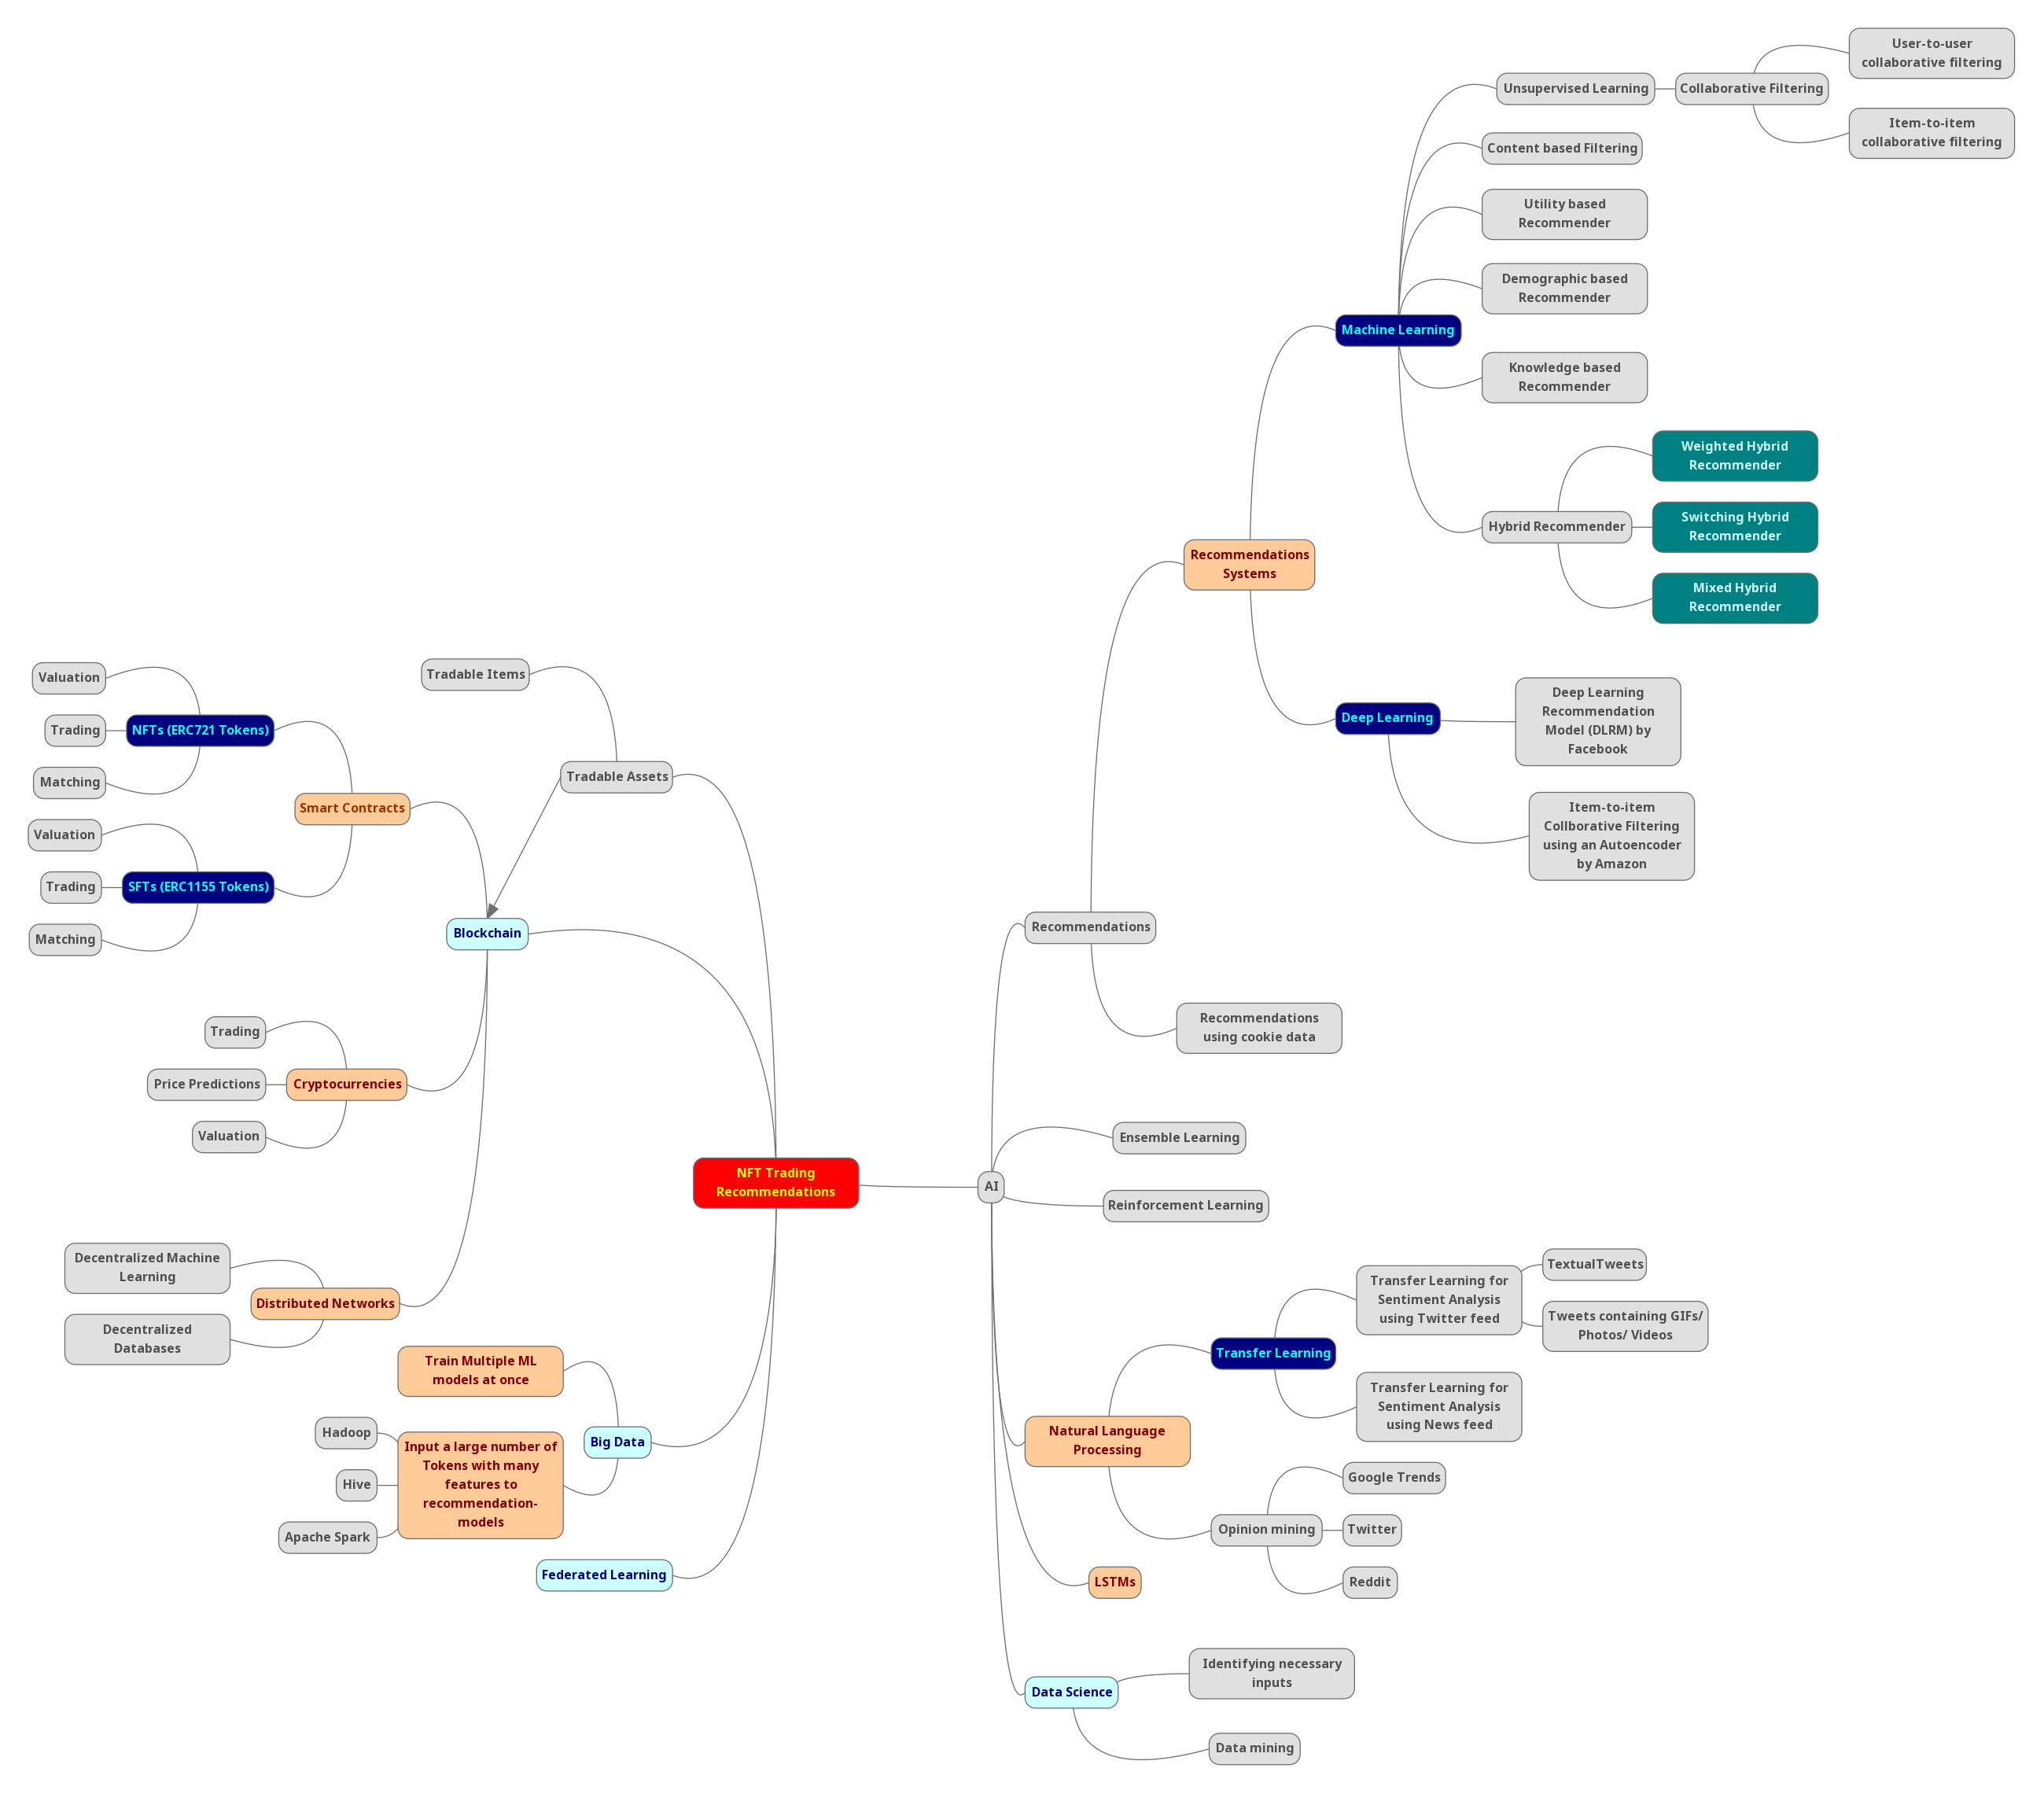
\includegraphics[width=10cm]{images/mind-map.png}
% \caption{Concept Map}
% \end{figure}


\section{Problem Domain}
% 3 pgs

% *** figure \autocite{noauthor_erc-721_nodate} - The comparison between NFT internet & the internet today can be used to show the value of NFTs in the thesis.

\subsection{ERC Standards}

The \gls{erc}-721 standard implements functionalities to transfer tokens from Blockchain accounts, to get the current token balance of an account, to get the owner of a specific token, the total supply of tokens available on the network, etc. Apart from the item itself, the creator can include metadata such as their signature in the NFT. What began on the Ethereum Blockchain with the ERC-721 standard has since been adopted by other Blockchains. 


\subsection{Benefits of NFTs for creators, collectors \& buyers}

% Benefits for creators, collectors, buyers
NFTs have a feature to allow a creator to make a certain percentage as royalty whenever the NFT is transferred to a new buyer. Since the items can be verified on the Blockchain, it also ensures that the original creator of the NFT can be tracked down and given due credit, any date in the future, no matter how many wallets it gets passed through \autocite{chevet_blockchain_2018}. Apart from the fact that a buyer can claim the right of ownership of the original item, they also get to financially support the creator. Ultimately, NFTs may gain value over time due to their scarcity. This gives collectors an additional advantage of being able to sell it for a higher price later on.

Creators of NFTs can also create "shares" for their NFT. This allows investors and fans to own a portion of an NFT without having to purchase the entire thing \autocite{noauthor_erc-721_nodate}.


\subsection{Recent news trends \& sales related to NFTs}

\begin{figure}[h!]
\centering
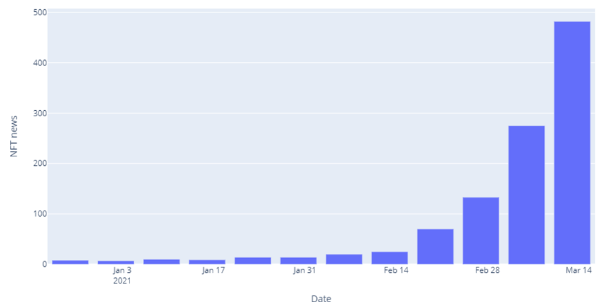
\includegraphics[width=10cm]{images/LR/NFT-news-trends.png}
\caption{News trends in 2021 related to NFTs \autocite{dowling_fertile_2021}}
\end{figure}

The above figure shows the increase in news trends related to NFTs since the start of 2021. It has been exponentially increasing and hitting headlines around the globe on a daily basis.
This depicts two factors. One is that NFTs are gaining more and more public attraction and acceptance. The second is that since there's a huge buzz among the public on social media and numerous web-sites, it makes sense to consider the opinions that are shared online by them.

\subsection{Value-driving factors in NFTs}

%  This para might be better-suited under Problem Domain
When considering ownership desire of \gls{nft}s, it is understood that the increase in price of an \gls{nft} has the possibility of being a factor to be considered when making a purchase.

\begin{quote} 
\centering 
\emph{"The value of an NFT is entirely determined by what someone else is willing to pay for it."}
\\
\raggedleft
\autocite{conti_what_2021}
\end{quote}

The value of an NFT has been identified to be heavily reliant on the public's acceptance of the item. Demand is expected to drive price rather than technical, or economic indicators which are the usual factors that affect stock prices and investor demand.

\begin{quote} 
\centering 
\emph{"Ultimately owning the real thing is as valuable as the market makes it. The more a piece of content is screen-grabbed, shared, and generally used the more value it gains. Owning the verifiable real thing will always have more value than not."}
\\
\raggedleft
\autocite{noauthor_erc-721_nodate}
\end{quote}

In addition to gaining value, due to the "non-fungible" nature of the item, it cannot be replicated. Similar to a Mona Lisa painting, popularity helps improve the value of the original and only the original is identified as the truly original painting with immense value, even though anyone can Google and get a copy of the painting.


\subsection{NFT Market places \& what they offer}
% Money in NFT & how markets have expanded (Open sea used by Reddit NFTs) and been funded.

\begin{figure}[h!]
\centering
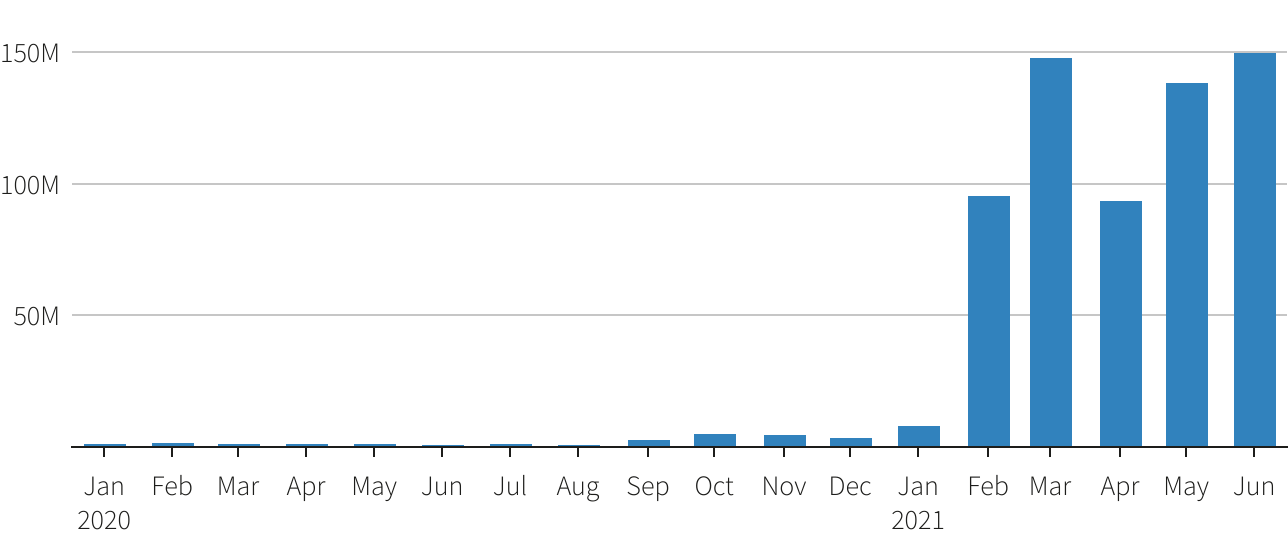
\includegraphics[width=12cm]{images/LR/NFT-sales-opensea.png}
\caption{Monthly Ethereum-based NFT token sales volume on the OpenSea marketplace, in USD \autocite{howcroft_nft_2021}}
\end{figure}

% Mention other Blockchains \& marketplaces that sell NFTs
% Market places - OpenSea, Rarible, and Grimes’ choice, Nifty Gateway


% -----------------
\subsection{Data mining NFTs}
% There're several factors that affect the desirablity of owning NFTs. When a person searches for NFTs he would be interested in knowing if the item is trending among the community - similar to the nature of crypto

% Add content from 5.2  Understanding factors that affect NFT Markets in proposal


% *** \/Related Work?
% CryptoKitties was one of the first NFT games & applications?
% Mention about NBA top-shot, Nike's CryptoKicks \autocite{}, artists work, etc. as industries that have stepped into the NFT craze and then...
% how the technology will evolve in the future.

% -----------------


% datamining NFTs....
% http://adilmoujahid.com/posts/2021/06/data-mining-meebits-nfts-python-opensea/

\subsection{Blockchain \& AI}
% Are Blockchain and AI a Perfect Combination? [WWW Document], n.d. . 101 Blockchains. URL https://101blockchains.com/blockchain-and-ai/ (accessed 7.23.21).

% AI & Blockchain - extremely important technologies for businesses. This lets me get to work with both domains \autocite{} AI & Blockchain article
% *** mention that since NFTs are also originating from computer science, it's important to understand the factors that affect the pricing and market created by them - here?

The very first study done examining the pricing of NFTs suggests that \emph{"prospects for future studies are potentially limitless, as at the beginning of any new market"} \autocite{dowling_fertile_2021}. As a future study, the author has suggested identifying if there's a fundamental model that drives the price determination in NFTs.

\subsubsection{Why create a Recommendations System for NFTs?}
In 2018 it was estimated that 35\% of Amazon's revenue \cite{naumov_deep_2019} is driven by Recommendation Systems. 75\% of Netlfix viewer activity \cite{vanderbilt_science_nodate} was also said to come from recommendations back in 2013. Therefore, it is clear that the use of a recommendation system that is catered toward the needs of potential \gls{nft} owners will help increase sales of \gls{nft}s, driving forward the adoption of this technology.


\subsection{Proposed architecture of a Recommendations System for NFTs}
By the requirements identified to purchase \& own \gls{nft}s, the author has proposes the following architecture to be followed in order to achieve the aim stated to be achieved in this research.

\begin{figure}[h!]
\centering
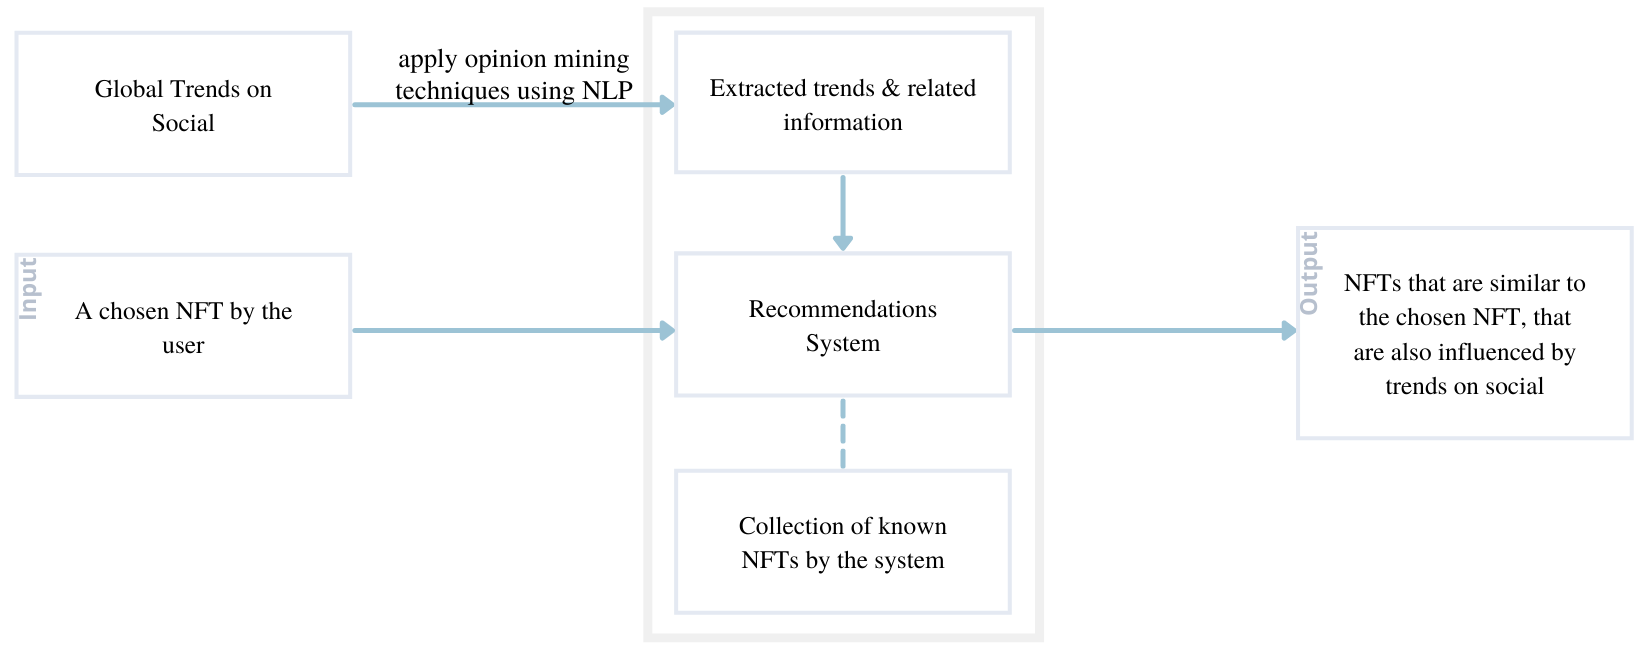
\includegraphics[width=0.9\textwidth]{images/LR/Proposed Architecture for domain.png}
\caption{Proposed architecture of a Recommendations System for NFTs \textit{(self-composed)}}
\label{fig:proposed-recommendations-architecture}
\end{figure}

As shown in figure \ref{fig:proposed-recommendations-architecture}, the proposed architecture is expected to make use of global trends extracted using social \gls{api}s. These can be from Twitter, Reddit, Google Trends or any other source that the user wishes to use. Once extracting relevant information using \gls{nlp}, the Recommendation System can then use this information to predict items that are relevant to the chosen item by the user and also those that have a possibility of getting influenced by trends on social.



\section{Existing Work}
% 4/5pgs+-
\subsection{NFT Recommendations Systems}

There is only one study previously done with related to recommending \gls{nft}s and that study also comes in the form of a blog article on \emph{OpenSea} \autocite{noauthor_what_2020}. The article considers the use of a basic \gls{ml} technique called \textbf{Multiple Regression} with data gathered from OpenSea.


This takes into account previous purchase patterns and NFTs held in wallets to predict whether another wallet carrying a similar combination is likely to own an NFT from a certain category in the future. The categories considered here are mostly collections created by specific well-known creators. Cryptokitties and ENS domains are a couple of examples for collections that have been taken into consideration.

As a final recommendation, this system is capable of presenting NFT categories. Since users can't purchase an entire category, they will have to go back to the process of picking which NFT to purchase in the recommended collection.

This doesn't take into consideration of current global trends and it will not take into account the creators' recognition. An NFT minted by Beeple or a major league like NBA are bound to capture more attention of buyers compared to an NFT minted by a person who hasn't gained any reputation in this space. The major concern with regarding this system is that the user must either enter his preferences manually or provide his wallet key, which holds all of his owned assets, in order to get a recommendation from the system. Although, getting a users' public key can by no means cause any threat of loosing the \gls{nft}s, it can be lead to lack of privacy, which is a tradition that the people into crypto-related assets have a tendancy to be concerned about.


\begin{quote} 
\centering 
\emph{"Crypto has a founding tradition of emphasizing freedom and privacy. Maybe because of this prevailing cultural trend, the NFT space does not have many recommender systems."} 
\\
\raggedleft
\autocite{noauthor_what_2020}
\end{quote}

As mentioned in the same blog post, this tradition is also been identified as a reason to why we have not yet seen much development related to Recommendation Systems in this space. Another reason could be because of the very recent spark in interest this domain has seen in recent times, as mentioned in the Problem Domain.


% \bigbreak


% ---------- 
\subsection{Crypto recommendations}

Since \gls{nft}s have a distant relationship with crypto assets, it is expected to be of help to understand how crypto assets are evaluated when opted for selection to comprehend how \gls{nft} assets could be evaluated. A study done related to a modelling framework that exposes this area of research \autocite{bartolucci_model_2020} assumes that two main features, namely security and stability can be used to determine the user-desire to own a specific crypto asset. 

Investor's attitudes towards assets’ features, information about the adoption trends, and expected future economic benefits of adoption have been simulated in order to predict the features of the assets that will most likely be adopted. The preference of investors are collected from an app, which calculates the overall state of the 'market'. Then, the app recommends to the user which crypto assets proposed by the user would be a sensible investment. Information about the adoption choice of other investors is considered when making this recommendation.

% limitation
The number of assets, investors and assets' features and investor preferences were fixed within the period of analysis. In a normal use-case scenario, it's highly likely that all these would fluctuate and evolve with the asset's adoption probabilities and expected returns. This revelation clarifies the fact that crypto related assets have a tendency to change with time, social acceptance and trends. Therefore, it is important to consider these factors when building a crypto-related Recommendations System.


\subsection{Opinion mining \& sentiment extraction based Recommendation Systems}

A \textbf{hybrid Recommendations System} \autocite{cheng_hybrid_2020} which utilizes \textbf{opinion \& sentiment extraction techniques from user reviews} to create preference profiles for movie recommendations, to enhance the quality of recommendations regardless of the rich or sparse nature of the dataset has been identified as one of the recent researches done towards pushing the limits of baseline recommendation models. The framework that has been designed here uses Collaborative Filtering as the base Recommendations model. The contribution of this research is applicable to the feature engineering stage of the system.

Sentiment analysis is applied on user-reviews to detect user-opinions about movies that were watched and reviewed by users. This data is used to create a user's preference profile, similar to what's created in Content-based filtering. The user's sentiment is identified as a step beyond traditional preference ratings.

% advantages
Due to its capability of dealing with insufficient data, the framework is able to produce recommendations that are more accurate and efficient than existing baseline methods. This proves that using public opinion in the feature engineering stage can enhance the quality of recommendations.

% limitations
Due to the fact that the semantic strategy of opinion extraction being generic, it is understood that it may not be ideal to identify different aspects in varied genres. Examples mentioned are, quality of sound may be of greater interest in action movies, while the story-line in dramas.
Slang, irony \& sarcasm haven't been taken into consideration when extracting user opinion.
A major limitation identified in most systems that rely on similar opinion mining systems is that they are very dependant on the text mining technique used. Another identified drawback in this research by the author is that, to establish a preference profile, a person must have posted reviews on previous movies. If not, those users won't be able to get recommendations. This can be identified as a concern in systems that are dealing with user's who care about their privacy.

\bigbreak

A \textbf{Deep Belief Network and Sentiment Analysis (DBNSA)} has been introduced to achieve data learning for recommendations \autocite{chen_user_2019} to enhance recommendations produced by baseline-recommendation techniques. This deep learning model  processes user comments to generate a possible user rating for user recommendations.

\begin{quote} 
\centering 
\emph{"Users usually transmit their decisions together with emotions."} 
\\
\raggedleft
\autocite{chen_user_2019}
\end{quote}

This research paper emphasizes the necessity of using user comments for recommendation systems since these comments contain a variety of emotional information that can influence the correctness and precision of recommendations.

% >>> feature engineering, pre-processing
Once applying sentiment analysis, a feature vector is created for the input nodes. A noise reduction procedure has been integrated into the system that deletes short comments, comments with no expression and false rating comments. This is used to improve the classification of user ratings. Finally, the DBNSA accomplishes data learning for the recommendations.

% advantages
The paper published claims to outperform baseline models in training loss, precision and recall when tested on Yelp \& Amazon datasets. When tested on the Trip-Advisor dataset, DBNSA had the best \gls{mse} training loss value \& recall. The research also mentions that DBNSA saves more time, while producing results with better accuracy compared to other baseline models.

% limitations
The main drawback that this paper points out is that the proposed system is not suitable \& ready for real-time testing. The authors of the paper have also shown interest in testing the proposed method with a faster Deep Learning algorithm. Similar to the previously mentioned system, sarcastic user-comments have not been taken into consideration here as well.
Out of the two recommendations models that were tested, \emph{libSVM} was identified to have higher accuracy value, \gls{mae} and F-score, while the \gls{mlp} had the highest precision value.

Since user relationships and timeline comments also affect the user's decision making, these can be used to find information from relatable timelines to solve the cold start problem.

\bigbreak
A \textbf{hybrid approach that combines techniques from content-based filtering, user-to-user collaborative filtering and personalize recommendations} \autocite{ayushi_cross-domain_2018} has been introduced to address the limitation of single domain analysis. Data sparsity and cold start problem have been pointed out as the addressed limitations. Movie domain knowledge has been used to generate recommendations for books \& music. 
After considering an array of supervised learning algorithms, the authors came to a conclusion that the Decision Tree classifier was found to give the highest accuracy.

% advantages
The use of data from multiple domains allows the system to generate higher accuracy in suggestions. Twitter sentiment has been used to present the user with an analysis of the recommendations produced, to help users in their decision making process.

% limitations
The drawback identified in the Recommendations System developed here is that Twitter sentiment is analysed, calculated and displayed only after showing the user recommendations.The author's suggestion is that only the items with positive sentiment could've been presented, at least results could've been bias towards positive sentiment.


\subsection{Price prediction using social-media trends}
%(crypt ~ NFT)
% Lamon, C., Nielsen, E., Redondo, E., n.d. Cryptocurrency Price Prediction Using News and Social Media Sentiment 6.

% (-)Abraham, J., Higdon, D., Nelson, J., Ibarra, J., 2018. Cryptocurrency Price Prediction Using Tweet Volumes and Sentiment Analysis 1, 22.
% ***this has why sentiment analysis isn't that important
% paraphrase quotes from this paper.

% While some studies present various methods to analyse news and social media sentiment, especially with the use of Twitter & Google Trends \autocite{},  

% ---------- 


% ---------- Price Prediction models

%  cite literature that tells NFTs behaviour compared to crypto - can be cited under Problem Domain as well
As mentioned under the Problem Domain section of this literature review, it is understood that \gls{nft}s have very little spill-over with other Crypto assets. However, knowing Crypto price prediction models is important since Wavelet coherence analysis indicates a co-movement between these two markets \autocite{dowling_is_2021}.
These models can be used separately on each NFT asset to anticipate the pricing with related to time, sales \& bids.
The author finds this research to be related to address the research gap in this thesis since an appropriate price prediction could be used to enhance \Gls{nft}  recommendations to users.

Past research suggests \textbf{a model which employs time series techniques, can predict the price for the next few days} by splitting the data into train and test runs \autocite{ferdiansyah_lstm-method_2019}.

% limitations
In terms of \gls{rmse}, the result is insufficient. The authors of this research have shown interest in testing out this method with modified \gls{lstm} layers by adding dropout and modifying the number of epochs. Using different instability data-sets can also be tried out to test how good the prediction results could get. 
Furthermore, sentiment analysis is also proposed as future work to be combined with the \gls{lstm} method. This could be used to identify how public sentiment 'causes the value of crypto to adjust, with related to past price-fluctuations.

% *** add a summary of all discussed systems here??


\section{Technological Review}
% unused technologies in domain can come here as well.
% 4pgs+-

Recommendations Systems allow users to identify trending items among a community, while being timely and relevant to the user's expectations. When the purpose of various Recommendation Systems differ, the required type of recommendations also differ from each use case. While one Recommendation System may focus on recommending popular items, another may focus on recommending items that are comparable to the user's interests. Content based filtering, user-to-user \& item-to-item Collaborative filtering and more recently; Deep Learning methods have been brought forward by the researches to achieve better quality recommendations.

Even though each of these methods have proven to perform well, there have been attempts to push the boundaries of their limitations. Following a wide range of methods, researches have tried to expand on the capabilities of standard recommendation systems in order to provide the most effective recommendations to users while being more profitable from a business's perspective. This has been achieved by taking a hybrid approach when building models and architectures for Recommendation Systems.

\subsection{Machine Learning based recommendation techniques}
There are several baseline techniques of Recommendations Systems that have been used by the biggest data-driven companies around the world.
% Explain about Collaborative, Content-based Filtering, Hybrid, Deep Learning Techniques, drawbacks, why baseline methods should be pushed forward using feature engineering, etc.
Among the many types of recommendation systems, \textbf{item-to-item Collaborative filtering} \autocite{linden_amazoncom_2003} has been the most successful technique for an extended period of time \autocite{smith_two_2017}, while user-to-user Collaborative filtering and Content based filtering have also had their own upsides. In order to take advantage of the relevant advantages of each method, Hybrid recommendation systems \autocite{geetha_hybrid_2018} were introduced. 

\subsection{Deep Learning based recommendation techniques}
% Deep learning models - 
% Embeddings Neu Embeddings?
In 2019, \textbf{Facebook} open-sourced a new categorical data-driven \textbf{Deep learning-based recommendation engine} \autocite{naumov_deep_2019, noauthor_we_2019}. This recommendation model was developed from the two perspectives of recommendation systems and predictive analytics. It made use of embeddings, two \gls{mlp}s, one sigmoid function \autocite{freudenthaler_factorization_2011} and a parallelization scheme to support large-scales of data.

In recent research done by \textbf{Amazon} \autocite{larry_history_2019} it is understood that when a timeline is considered for recommendations, an \textbf{\emph{Autoencoder} Deep Learning model} is capable of Recommending the best possible combination of movies to users.


\subsection{Concerns about progress in Recommendation Systems}
In several research \& review papers, it has been brought to sight that Deep learning techniques in the area of recommendation systems have failed to live up to the expectations compared to the advancements in Computer Vision, Speech Recognition \& Natural Language Processing domains \autocite{choi_local_2021}. The results that have been published presenting advancements in the Recommendation Systems domain using Deep learning techniques have not been very convincing for the majority of use cases. Many standard Machine learning \& regression techniques have been able to outperform systems created using Deep learning models in terms of recommendations. As highlighted in past reviews \autocite{dacrema_are_2019} it is understood that Deep learning models have been used as baseline methods for evaluating new Deep learning models. Thus, when looking back at older Machine learning techniques, they haven't been making any improvement in many cases. As a result, many of the work related to Recommendation Systems using Deep learning techniques have been giving poorer recommendations, for higher computational power.


A study conducted in 2019 questioned if we are really making any progress with Deep Learning models in the domain of Recommendations \autocite{dacrema_are_2019}. In a more recent study researches tried to understand similarities and advantages of using \textbf{MLP (Multi Layer Perceptron)} versus \textbf{dot product} \autocite{rendle_neural_2020}. Similar to many Deep learning approaches, it was understood that MLP weren't necessary unless the dataset was too large or the embedding dimension was very small. A dot product was identified as a better choice since it was efficient to a satisfactory extent.

\subsection{How to choose the ideal algorithm for a Recommendations System?}

A general application of a Recommendation System will come in a business use case, where companies focus on maximizing profits for minimum expenses. In a scenario like that, it would make more sense to choose a cheaper model that gets the job done to a satisfactory level. Dot products offer a significant advantage over MLPs in terms of inference cost due to the availability of efficient maximum inner product search algorithms. Since MLPs are too costly to use in production environments, the better default choice in most cases would be the dot product approach that uses Machine Learning techniques with Matrix Factorization.
A variation that combines the MLP with a weighted dot product model, named \textbf{\emph{neural matrix factorization (NeuMF)}} is also explored in this research. But, that too is deemed to be outperformed by the dot product method.

One of the major limitations identified related to dot product in this study is that, learning a dot product with high accuracy for a large embedding dimension required a large model capacity. This may also require more computational resources. Therefore, it would be advisable for Data Science engineers to consider both approaches based on the requirements \& data of the system that they're planning to work on.

% *** cite ensemble techniques of recommendation systems

\subsection{Architectures of Recommendation Systems that integrate opinion mining techniques}
There have been many attempts to expand the capabilities of Recommendations by making use of public opinion. Collaborative Filtering was one approach to achieve that. Another identified approach was to make use of user-data on social media. This has been integrated into Machine Learning-based Hybrid Recommendation Architectures in many ways. In the figure \ref{fig:recommendation-opinion-mining-enhancements}, the author tries to elaborate on the possible technical contribution brought forward in this research.

\begin{figure}[h!]
\centering
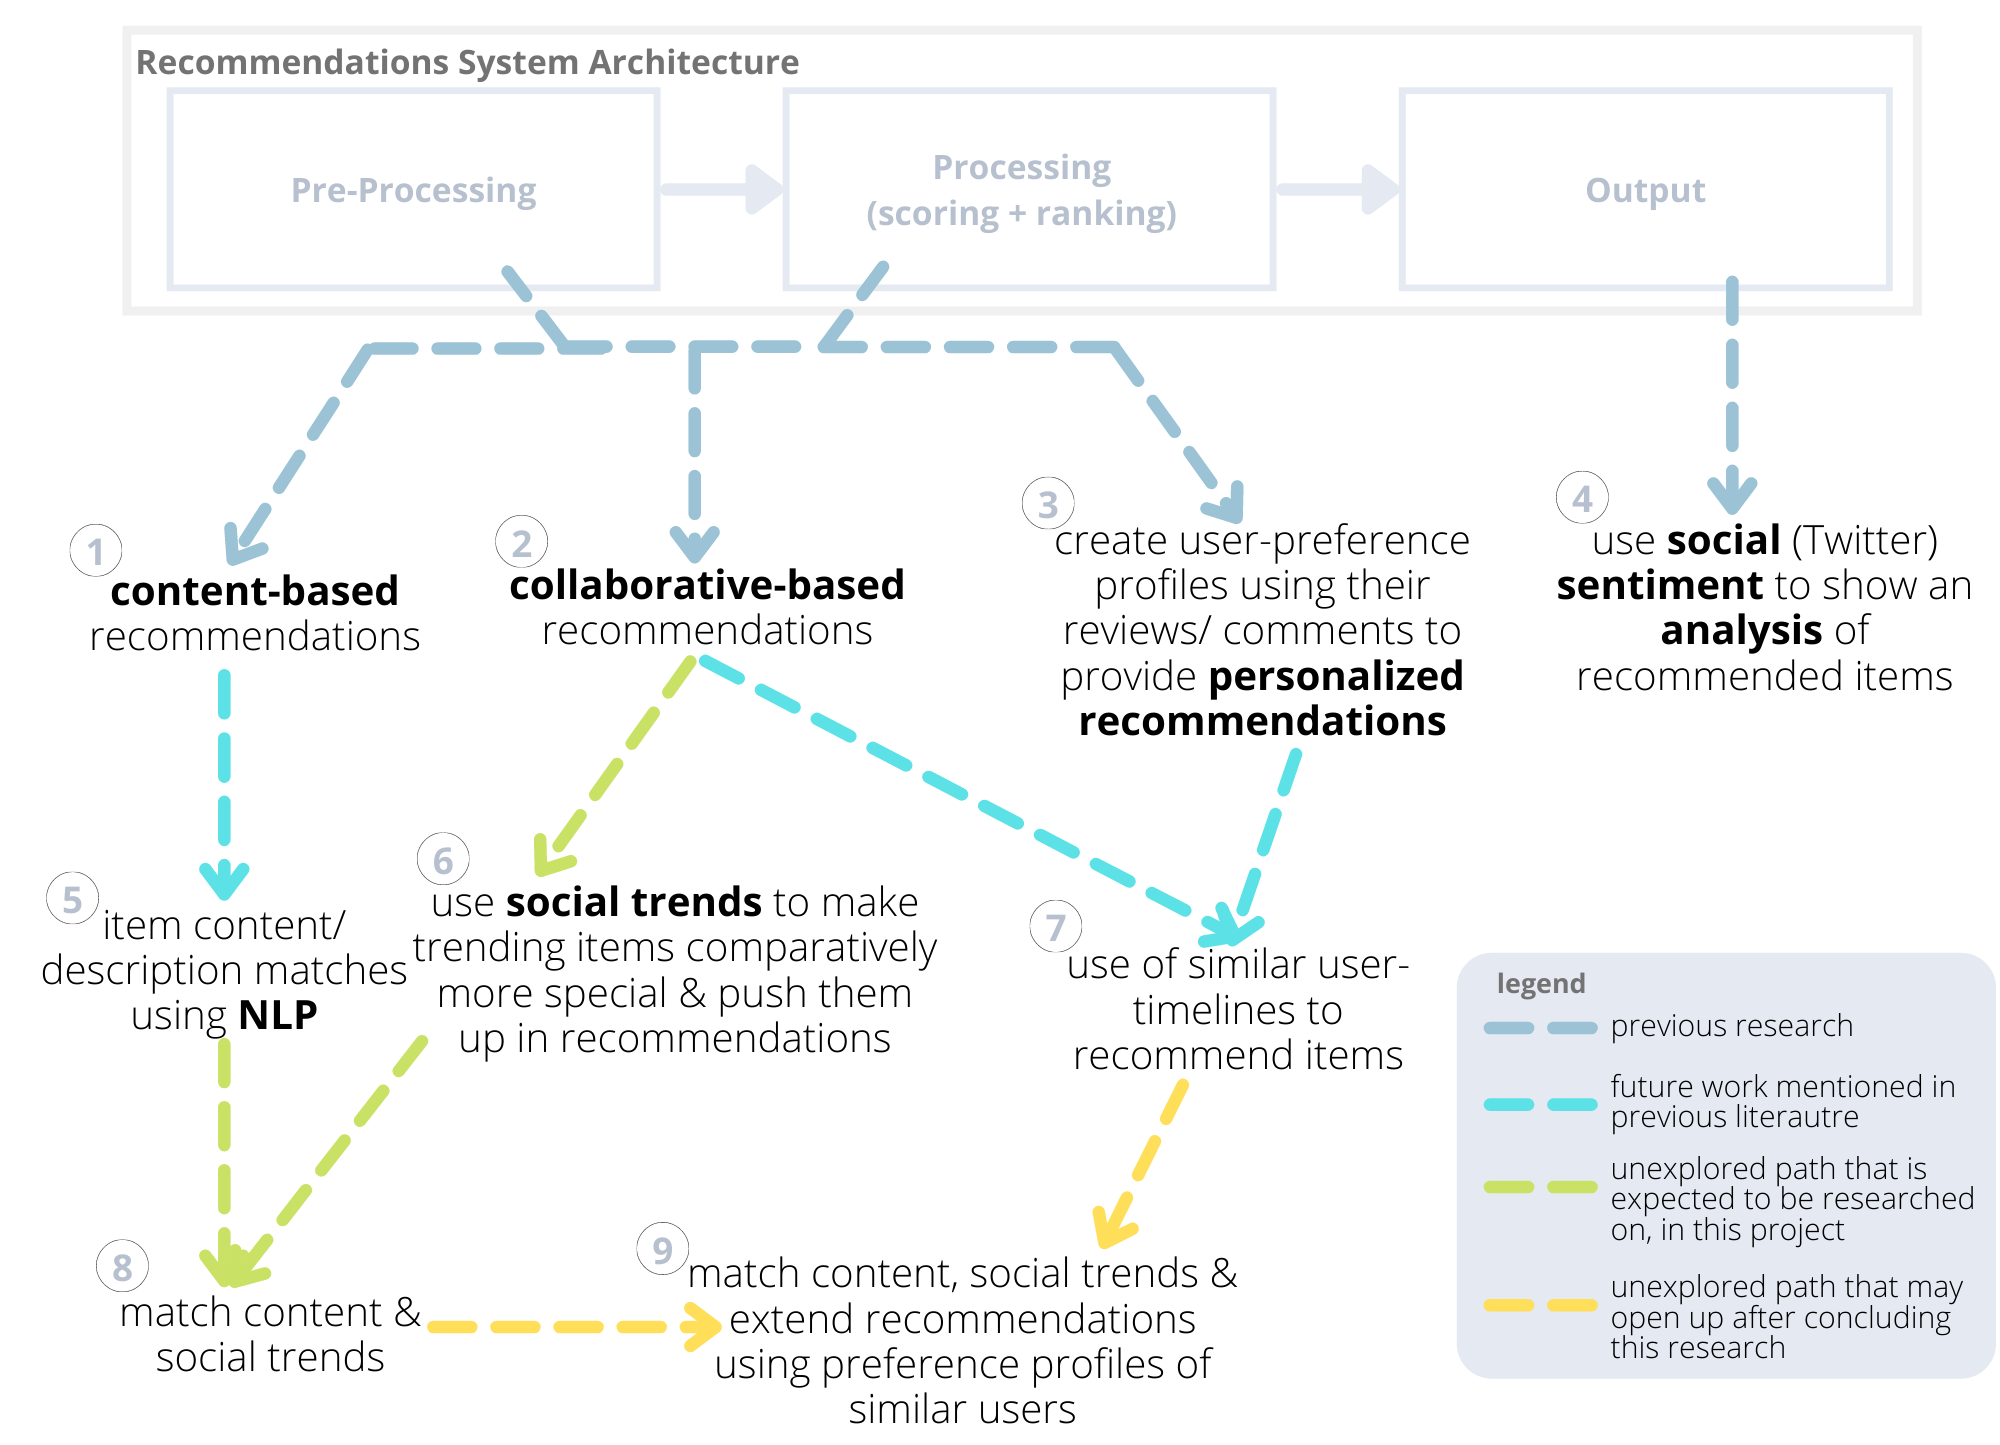
\includegraphics[width=\textwidth]{images/LR/Enhanced Recommendation Systems.png}
\caption{Enhancements done to Recommendation Systems using opinion mining techniques \textit{(self-composed)}}
\label{fig:recommendation-opinion-mining-enhancements}
\end{figure}

The figure \ref{fig:recommendation-opinion-mining-enhancements} shows the identified possible points of integration of opinion mining techniques to a Recommendations System.
1, 2 \autocite{linden_amazoncom_2003, larry_history_2019}, 3 \autocite{cheng_hybrid_2020} \& 4 \autocite{ayushi_cross-domain_2018} techniques have been already applied as identified in past literature, while the 7\textsuperscript{th} technique has been mentioned as a possible future work from the 3rd technique \autocite{chen_user_2019}. Method 5 hasn't been explicitly attempted in recent literature with respect to Recommendation Systems, but the data science models used aren't expected to require a lot of tweaking to achieve it, after the feature engineering step is being taken care of.

Method 6 has not been identified in previous literature and is expected to align better with the desires circulating the \gls{nft} market-space. This can be extended to method 8. Finally, if methods 7 \& 8 turn out to give promising results, method 9 would be the next step to provide a completely new personalized recommendations architecture that integrates social media trends that are related to the content of the items.

\subsection{NLP techniques that can be applied to support integration of opinion mining into Recommendation Systems}
% NLP techniques that can be applied (Sentiment analysis, word/ noun matching)

% \autocite{hu_reviewer_2020} - This paper's related work section can be used to prove why sentiment analysis is needed for recommendations.

% >>>> (can add points from this to why senitment-aware recommendation systems are useful) cite: Zhang, W., Xu, M., Jiang, Q., 2018. Opinion Mining and Sentiment Analysis in Social Media: Challenges and Applications, in: Nah, F.F.-H., Xiao, B.S. (Eds.), HCI in Business, Government, and Organizations, Lecture Notes in Computer Science. Springer International Publishing, Cham, pp. 536–548. https://doi.org/10.1007/978-3-319-91716-0_43


\subsection{Practices to be followed to optimize the usage of gathered opinions}
When considering multiple opinions related to a specific topic/ item, they can be combined into one document and processed rather than processing each opinion one by one \autocite{nah_opinion_2018}. When doing so, it would be good to have an impact score of each document to make sure that recommendations are biased appropriately towards the opinions of the majority with consideration of the users' opinions.



\section{Review of Evaluation Approaches}
When evaluating Recommendation Systems, we may examine the outcomes produced by the system in two ways.
The first way would be identifying if the system is capable of recommending items that a user may use. The second method would be to identify if the system is capable of recommending items that a user will choose/ use.

\bigbreak
The first way to evaluating the outcome can be done utilizing current data and pre-identified conditions. For the second approach, the evaluation algorithm would require feedback from the public. This can be done by having open beta testing. It would take more time \& effort, but it will be capable of evaluating a system qualitatively on the final goal instead of a possibility.

If we look at evaluating this system from an expected-output performance point of view, P@K, also identified as Top-N strategy in several literature is the most common method of evaluating a Recommendations System.
This measure and the benchmarking methods that have been mentioned below can be used to \textbf{quantitatively} evaluate Recommendation Systems.

Apart from these metrics, quality-of-service measures such as CPU \& Memory usage can be considered for evaluation as well. 

In the review questioning the advancements of Recommendation Systems, \autocite{dacrema_are_2019} the author mentions that the lack of used datasets and code-bases hinder the ability to properly benchmark and evaluate new research related to Recommendation Systems. The importance of reproducibility of research related to Recommendations Systems have future been elaborated in reviews that follow \autocite{dacrema_troubling_2021, ferrari_dacrema_critically_2020, dacrema_methodological_2020}.


\subsection{Benchmarking}
The following are some benchmarking strategies that can be used to assess the performance of Recommendation Systems.

\begin{longtable}{|p{0.2\linewidth}|p{0.4\linewidth}|p{0.28\linewidth}|} 
\caption{Benchmarking techniques for Recommendation Systems}
\label{tab:benchmarking-techniques-table}\\
\hline
Measure & Description & Objective Orientation \\ 
\hline
\gls{mae} & Measures the average absolute deviation between a predicted rating and the user’s true rating, overall the known ratings. & \multirow{2}{=}{Negatively oriented. Lower, the better.} \\ 
\cline{1-2}
\gls{rmse} & A variant of MAE emphasizes large errors by squaring them. &  \\ 
\hline
Precision & The percentage of items in the recommended list that are assessed to be relevant to the user (i.e. it represents the probability that a selected item is relevant). & \multirow{2}{=}{Positively oriented. Higher, the better.} \\ 
\cline{1-2}
Recall & The ratio of relevant items presented by the system to the total number of relevant items available in the items in the system. &  \\
\hline
\end{longtable}

\gls{mae} \& \gls{rmse} are used to measure the accuracy of predicted user-ratings (1-5 star ratings) per item, per user. Precision \& recall are used to measure if the system successfully predicts which items the user will select or consume \autocite{dayan_recommenders_2011}.

\bigbreak
A common test dataset is required in order to consider the results produced by these methods to be valid. Since there’s no previous \gls{nft} Recommendation System found in research, the author will not be able to conduct a comparative benchmark analysis on the proposed system.

The benchmarks produced by this system will be made available public together with the used datasets in order to allow future researchers to evaluate new Recommendation Systems in this domain.


% \section{Tools}
% 3/4pgs+-
% \subsection{NLP libraries that can be used for opinion mining purposes}
% RNN based - Spacy/ NLTK
% transformer-based - hugging face

% mention pros & cons and why it will be good to use one of the two based on the affect it has & the accuracy

% \subsection{Libraries that can be used for web-scraping purposes}

\section{Chapter Summary}
% 1/2 pg